\section[Windows Internals]{Windows Internals}

To understand memory forensics on Windows, knowledge about Windows Internals is necessary, from the memory model to some kernel design. In this section, we will give the reader some technical details on Windows' design.

\subsection[Memory model]{Memory model}

We start by exploring the Windows memory model, and more importantly, the Windows kernel memory model. Windows by default use page size of 4KB, the virtual address space for each process is 2GB for the 32-bit version and 8TB for the 64-bit version. The system address space is 2GB for the 32-bit version and 248TB for the 64-bit version. For every process, when run, can see both its own address space and the system space, but access to the system space is restricted. A typical 32-bit process can have a 2GB space for itself and a 2GB space of the system, makes a total virtual memory space 4GB. The system space, refer to as the kernel space, contains the OS kernel objects and the currently running drivers and kernel application. The kernel space uses \textit{pools} to manage objects allocation and deallocation. Windows has two types of pool, one that is \textit{pagable}, can swap out to disk, called \textit{paged pool} and the other \textit{non-paged pool}. The size of these two types of pools on Windows 10 can be referred through the Table~\ref{tab:poolsize} \cite{memorylimit}. Because many parts of the OS is not used often, Windows can swap those pages out to make more space. However, some information will always remain in the non-paged pools.

\begin{table}[h]
\centering
\caption{Pool size on Windows 10}
\label{tab:poolsize}
\begin{tabular}{l p{5cm} p{5cm} }
\toprule
\textbf{Pool Type} & \textbf{Limit on 32-bit} & \textbf{Limit on 64-bit} \\[5pt] \hline
\rule{0pt}{\normalbaselineskip}
Paged Pool & 384 GB or system commit limit, whichever is smaller & 384 GB or system commit limit, whichever is smaller \\[5pt]
Non-paged Pool & 75\% of RAM or 2 GB, whichever is smaller. & RAM or 128 GB, whichever is smaller (address space is limited to 2 x RAM) \\
\bottomrule
\end{tabular}
\end{table}

The memory pool is a bitmap, an array of bits. Windows will return the pointer and size when asked for space in the pool (chunk). Windows keeps track of chunks in the pool. At first, there is only one chunk (the pool itself). When the user asks for space, Windows will split the chunk into two, one for the user and one left unused, Windows will keep splitting the unused space in the pool and return to the user for any allocation requested. Upon deallocation, Windows will merge unused chunks into one. Consider the code in Listing~\ref{lst:basicpool} for a basic example of pool allocation.

% TODO: Picture

Each chunk will have a \texttt{POOL\_HEADER} field on the top to denote the content of the chunk. \texttt{POOL\_HEADER} has a size field (\texttt{BlockSize}), a previous size field (\texttt{PreviousBlockSize}), and a tag (\texttt{POOL\_TAG}). Tag is a four-byte character that Windows and Driver writer use to denote the data stored in the chunk. In Table~\ref{tab:pooltag}, we listed some typical structure with its tag.
\newpage
\lstinputlisting[language=cpp,caption={Basic Pool Algorithm},label={lst:basicpool}]{code/basic_pool.cpp}

\begin{table}[h]
\centering
\caption{Some pool tags and their corresponding structure}
\label{tab:pooltag}
\begin{tabular}{lll}
\toprule
\textbf{Structure}     & \textbf{Structure Name}   & \textbf{Pool Tag} \\ \hline
Driver Object & \texttt{\_DRIVER\_OBJECT} & Driv     \\
File Object   & \texttt{\_FILE\_OBJECT}   & File     \\
Process       & \texttt{\_EPROCESS}       & Proc     \\
TCP endpoint  &                  & TcpE     \\
TCP listener  &                  & TcpL     \\
Thread        & \texttt{\_ETHREAD}        & Thre     \\
UDP endpoint  &                  & UdpA     \\
\bottomrule
\end{tabular}
\end{table}

\subsection[EPROCESS and ETHREAD]{EPROCESS and ETHREAD}

Windows has a special structure that contains process information called \texttt{\_EPROCESS}. This structure is created every time when a new process spawns and located inside a non-paged pool with tag \textit{Proc}. If we have a reference to one \texttt{\_EPROCESS} we might follows \texttt{LIST\_ENTRY ActiveProcessLinks}, a doubly-linked list pointer, to find other \texttt{\_EPROCESS} of different process Figure~\ref{fig:eprocesslink}. However, because a normal user can access this structure by calling \texttt{PsLookupProcessByProcessId} one may edit the doubly linked list to remove itself from the list chain as can be seen in Figure~\ref{fig:dkom}.


\begin{lstlisting}[language=cpp,caption={LIST\_ENTRY},label={lst:listentry}]
typedef struct _LIST_ENTRY {
      struct _LIST_ENTRY *Flink;
      struct _LIST_ENTRY *Blink;
} LIST_ENTRY, *PLIST_ENTRY, PRLIST_ENTRY;
\end{lstlisting}

\begin{figure}[H]
\centering
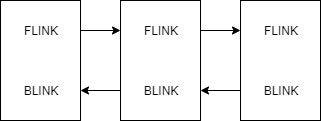
\includegraphics[scale=0.6]{images/eprocess_link.png}
\caption{EPROCESS linking}
\label{fig:eprocesslink}
\end{figure}

\begin{figure}[H]
\centering
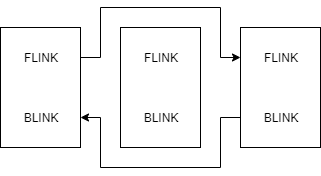
\includegraphics[scale=0.6]{images/dkom.png}
\caption{EPROCESS linking modified}
\label{fig:dkom}
\end{figure}

A process in Windows is composed of threads. For example, a process loading a library will have the library run as a thread. Every thread will have a kernel object inside the non-paged pool called \texttt{\_ETHREAD}. From an \texttt{\_ETHREAD} by calling \texttt{IoThreadToProcess}, Listing~\ref{lst:threadtoprocess}, one can get the parent \texttt{\_EPROCESS}. An \texttt{\_EPROCESS} has a doubly-linked list of \texttt{\_ETHREAD} in \texttt{LIST\_ENTRY ThreadListHead} to list threads of a process.

\begin{lstlisting}[language=cpp,caption={IoThreadToProcess},label={lst:threadtoprocess}]
PEPROCESS IoThreadToProcess(
  PETHREAD Thread
);
\end{lstlisting}

\subsection[KDBG]{KDBG}
\label{sec:kdbg}

KDBG short for \texttt{Kernel Debugger Block} is one of the commonly used structure when analyzing a memory artefact of Windows. It was created to easy debugging process for developers when writing OS or kernel drivers as this structure contains pointers to other structures. One pointer contained in KDBG is \texttt{PsActiveProcessHead} which is a pointer to an \texttt{\_EPROCESS}. As previously mentioned, we can walk the list of \texttt{\_EPROCESS} to enumerate all processes.

\subsection[Windows dump file]{Windows dump file}

Windows provides a dump file to contains compressed memory data. This file is created by Windows when an error in kernel occur. Third-party tools can dump the memory on running machine, for example, DumpIt, FTK Imager. This file structure is not documented but Schuster \cite{dmpfile} has written a guide to the file structure. Another dump file type is minidump file which is documented by Joachim \cite{mdmpfile}. These dump files are commonly used to preserve the system memory state for analysis.

\subsection[Process injection]{Process Injection}
\label{sec:processinjection}

Process injection is a technique to inject a process to another running process. In 2019, Amit Klein and Itzik Kotler gave a talk at the US Blackhat conference about the topic \cite{processinjection}. The research is done on Windows 10 x64, and they tried to systemize the process injection techniques. Some techniques could still be used although Windows 10 has better security than previous Windows version. A process injected will be more stealthy since the system can only see the parent process. This method is often used by malware to make their process hidden from the system. For any process spawn, a thread with \texttt{\_ETHREAD} is always created, and investigators often rely on this to detect hidden threads.

% \subsection[API hooking]{API hooking}

% TODO
